\documentclass[paper=a4, fontsize=11pt]{scrartcl} %twocolumn, 

\usepackage[utf8]{inputenc} % Use 8-bit encoding that has 256 glyphs

%\usepackage{fourier} % Use the Adobe Utopia font for the document - comment this line to return to the LaTeX default
\usepackage[english]{babel} % English language/hyphenation
\usepackage{amsmath,amsfonts,amsthm, amssymb} % Math packages, use \sim to get tilde

\usepackage{graphicx} % Required for including pictures

\usepackage{booktabs} % Allows the use of \toprule, \midrule and \bottomrule in tables for horizontal lines

%----------Pasting Code---------------

\usepackage{listings} % \usepackage{listings} For inserting code into the document
% Using \usepackage{listingsutf8} for multi-byte encoding of source code

\lstset{breaklines = true, 
numbers = left, 
commentstyle = \color{mygreen}, 
keywordstyle = \color{blue}, 
stringstyle = \color{mymauve},
showstringspaces = true,
basicstyle=\footnotesize
}
%inputencoding = utf8, 
%extendchars = \false

%\usepackage{minted}
\usepackage{color} %for syntax highlighting

\definecolor{mygreen}{rgb}{0,0.6,0}
\definecolor{mygray}{rgb}{0.5,0.5,0.5}
\definecolor{mymauve}{rgb}{0.58,0,0.82}

%------------END--------------

\usepackage{float} %for aligning figures

\usepackage{wrapfig} %for using wraptable or wrapfig

\usepackage{caption}
\usepackage[l2tabu]{nag}

%\usepackage[nottoc]{tocbibind} %to include the bibliography in the contents

\usepackage{verbatim} %use \begin{comment} and \end{comment}. For more complex tasks, check out package:comment

\usepackage{bm} % for printing greek symbols in bold, use \boldsymbol\varepsilon

\usepackage{rotating} % for rotating tables
\usepackage{longtable} % for long tables, 

\usepackage{subcaption} %for supressing table numbering in subtables
\usepackage{makecell} %for multiple lines in a table, enclose the cell value in \thead{A \\ B}

\usepackage{lscape} %for rotating the page with the long table

\usepackage{todonotes} %add TODOs by putting the text in \todo{}

\usepackage{csquotes} %use \begin{displayquotes} to enter a quote

\usepackage{adjustbox} % to adjust the size of long tables if they go beyond the page

% for changing the nature of urls
%\usepackage[hidelinks]{hyperref} %hides hyperlinks
\usepackage[linktoc = none, linkbordercolor	={0 1 0}]{hyperref}

% custom commands
\newcommand{\mytilde}{\raise.17ex\hbox{$\scriptstyle\mathtt{\sim}$}}

\usepackage{fancyhdr} % Custom headers and footers
\pagestyle{fancyplain} % Makes all pages in the document conform to the custom headers and footers
%\fancyhead{} % No page header - if you want one, create it in the same way as the footers below
\fancyhead[L]{}
\fancyfoot[L]{} % Empty left footer
\fancyfoot[C]{\thepage} % Page numbering for right footer
\fancyfoot[R]{} % Empty right footer
\renewcommand{\headrulewidth}{0pt} % Remove header underlines
\renewcommand{\footrulewidth}{0pt} % Remove footer underlines
\setlength{\headheight}{13.6pt} % Customize the height of the header

\numberwithin{equation}{section} % Number equations within sections (i.e. 1.1, 1.2, 2.1, 2.2 instead of 1, 2, 3, 4)
%\numberwithin{figure}{section} % Number figures within sections (i.e. 1.1, 1.2, 2.1, 2.2 instead of 1, 2, 3, 4)
%\numberwithin{table}{section} % Number tables within sections (i.e. 1.1, 1.2, 2.1, 2.2 instead of 1, 2, 3, 4)

\setlength\parindent{5pt} % Removes all indentation from paragraphs - comment this line for an assignment with lots of text

\graphicspath{{"/home/ad/Desktop/KUL Course Material/Statistical Modelling/R programming/"}} % Specifies the directory where pictures are stored

%----------------------------------------------------------------------------------------
%	Some Tips For Using This Template
%----------------------------------------------------------------------------------------


\begin{comment}

\end{comment}

%----------------------------------------------------------------------------------------
%	TITLE SECTION
%----------------------------------------------------------------------------------------

\rhead{Akshat Dwivedi}
\lhead{Statistical Modelling}
%\rfoot{\begin{picture}(0,0) \put(-45,-100){\includegraphics[width=3cm]{KU_LeuvenFR}} \end{picture}}
\newcommand{\horrule}[1]{\rule{\linewidth}{#1}} % Create horizontal rule command with 1 argument of height

\title{	
\normalfont \normalsize 
\textsc{\Large KU Leuven} \\ [30pt] % Your university, school and/or department name(s)
\horrule{0.5pt} \\[0.4cm] % Thin top horizontal rule
\huge Statistical Modelling: Final Assignment \\ % The assignment title
\horrule{2pt} \\[0.5cm] % Thick bottom horizontal rule
}

\author{Akshat Dwivedi (Student Number: blah blah)\\
\\
Instructor: Prof. Gerda Claeskens} % Your name

\date{June 1, 2016} % Today's date or a custom date

\pagenumbering{arabic}

%--------------------------------------------------------------------------------

\begin{document}

\maketitle % Print the title

%\tableofcontents

\thispagestyle{empty}
\clearpage
\setcounter{page}{1}

%\listoftodos %makes a list at the top of the document with TODOs

% Begin writing here:

\section{Part A}

The dataset used in this part of the project contains information about Belgian municipalities for the year 2014. Our aim is to study how and whether these variables help explain the number of births in the municipalities. The variables in the dataset are: province, income, zero\_income (individuals that do not pay taxes), population density, num. of marriages, num of divorces, population on the first and last day of the year, deaths, incoming and outgoing  internal as well as international migration, number of nationality changes and the response variable which is number of births per 1000 (also known as crude birth rate (CBR)) inhabitants.

\subsection{A.1}

The average number of births per 1000 inhabitants and the average number of international migrants per province is given in table \ref{average}.

\begin{table}[h]
\centering
\begin{adjustbox}{max width=\textwidth}
\begin{tabular}{c|ccccccccccc}
\hline
Province & Antwerp & \thead{Flemish \\ Brabant} & \thead{West \\ Flanders} & \thead{East \\ Flanders} & Hainaut & Liege & Limburg & Luxembourg & Namur & \thead{Walloon \\ Brabant} & Brussels \\
\hline
\thead{Num. of \\ Incoming \\ International \\ Migrants} & 2575 & 1263 & 1502 & 1791 & 1875 & 3265 & 3425 & 2200 & 2854 & 2872 & 4020 \\
\hline
\thead{births \\ per 1000} & 13.77 & 12.82 & 12.20 & 12.46 & 12.39 & 14.61 & 15.44 & 14.08 & 15.82 & 13.83 & 20.17 \\
\hline
\end{tabular}
\end{adjustbox}
\caption{Section A.1: Average number of incoming international migrants and births per 1000 (crude birth rate) for each province in Belgium.}
\label{average}
\end{table}

We wish to test whether the provinces Flemish Brabant and Brussels have similar number of incoming international migrants and births per 1000. For Brussels, we have 3 observations in our dataset and for Flemish Brabant, we have 13 observations. Since 13 is quite small and 3 is too small, a t-test is out of the question. It would be unreasonable to assume that the distributions are normal with such a low sample size. We can perhaps use a nonparametric test such as Mann-Whitney U test (for 2 samples) or Kruskal-Wallis (extension of Mann-Whitney for more than 2 groups), however, either way, 3 observations in one group is going to be problematic for drawing inferences. This small number is due to the seed chosen for obtaining a subset of the full dataset for analysis. We present the results from these tests below but these are not desirable since the CIs will be too wide. For this, we used the Mann-Whitney test which is a two-sample test for difference in location with $H_0: \mu_1 - \mu_2 = 0$ vs $H_a: \mu_1 - \mu_2 \neq 0$. The sample sizes for each of the groups is $n_1 = 13$ (Flemish Brabant) and $n_2 = 3$ (Brussels).\\ 

For the variable births per 1000, the estimated difference in location is -9.0207 (95\% CI: [-14.134, 0.359]) with a $p-$value of 0.05714. The effect size reported here is negative, which means that the average birth rate for Flemish Brabant is lower than than the average birth rate for Brussels although this difference is not statistically significant. On the other hand, for the number of incoming international migrants, the estimated difference in location is -2582 (95\% CI: [-7134, 431]) with a $p-$value of 0.05714. The effect size is negative which means the average number of international incoming migrants is lower in Flemish Brabant compared to Brussels (as is expected), however, this difference is not statistically significant. The estimated CIs are really wide, most likely due to a small number of sample sizes for each of the groups and hence, the conclusions about the differences in group means are not particularly precise. \\

As an aside, we tried this on the full dataset with $n_{vlaams}=65$ and $n_{BRU}=19$ and this was enough to narrow the CIs and it was observed that the conclusions drawn above are the same (birth rate ES: -2.951, 95\% CI [-7.61,-1.34], $p = 0.002$; international migration ES: -1609, 95\% CI [-2328, -290], $p = 0.016$; $p-$values are two sided).

\subsection{A.2}

In this part we fit a flexible regression model $log(BirthPer1000) = f(Intl\_Mig) + \varepsilon$, $\varepsilon_i \sim \text{Poisson(BirthPer1000\_i)}$ (where $\text{BirthPer1000}_i = exp(\beta\text{Intl\_Mig}_i))$ is the link function for the Poisson model) using penalized smoothing splines. The fitted model using splines has $\approx 5$ degrees of freedom ($df = 5.456$). Inspecting the fitted curve, we pick (50, 400, 1300, 9500) as the four knots for the linear spline basis function. The fitted spline and the parametric line (GLM with Gamma errors and log link) is given in figure \ref{4knots}.

\begin{figure}[ht]
\centering
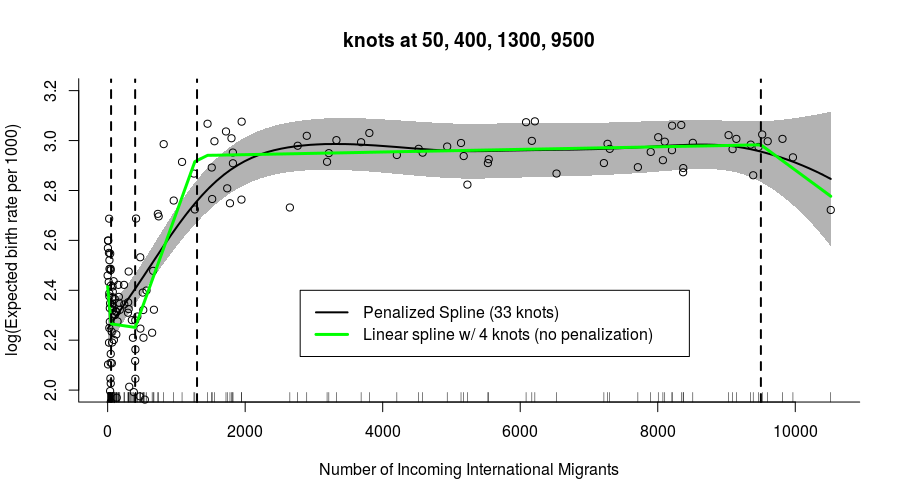
\includegraphics[width = 0.9\textwidth]{4knots.png}
\caption{Section A.2: Fitted spline model with birth rate per 1000 as response and International Incoming Migrants as predictor. The black line is the spline fit; the green line is from the parametric (piecewise linear) fit with knots at (50,400,1300,9500); the black dashed lines indicate the positions of the knots. The model does not seem to fit well on $x \in [0, 500]$ as most of the observed values are far from either of the fitted values.}
\label{4knots}
\end{figure}

We test which knots to keep in the parametric model using 1) likelihood ratio tests and 2) information criteria. Based on the model summary, we use the likelihood ratio test between the model with these 4 knots and the model with knots only at 400 and 1300. The resulting $\chi^2 = 4.825$ with $df = 2$ and the corresponding $p$-value is 0.089. This shows that the likelihood does not differ much between the two models. The BIC for model with 2 knots is 699.42 vs 694.22 for the model with 4 knots. Based on these, it is clear that the knot at 9500 can be removed, however, it is not entirely evident whether the knot at 50 should be removed or not. We decide to remove the knot at 50 and only keep the knots at 400 and 1300, which results in a piecewise linear model. The equation for the chosen model is
$$ \text{log}(y_i) = \beta_0 + \beta_1 x_{1i} + b_1(x_{1i} - 400)_+ + b_2(x_{1i} - 1300)_+ + \varepsilon_i $$

with $\varepsilon_i \sim \Gamma(\theta, k)$ and y$_i$ = birthRatePer1000$_i$ and x$_1$ is number of incoming international migrants. 

\subsection{A.3}

In this section we fit an additive model with Income (in 1000s euros) and Zero Income (number of people that did not pay tax) to the response births per 1000 people (crude birth rate) using penalized smoothing splines using the spm function from the R package SemiPar. The equation for this model is 
$$\text{log}(\text{birthsPer1000}_i) = \beta_0 + f(\text{Income}_i) + g(\text{ZeroIncome}_i) + \varepsilon_i $$ where $\varepsilon_i  \sim \text{Poisson}(\lambda_i)$; $\lambda_i = \text{birthsPer1000}_i$.\\

The output from the fitted model shows that the estimated degrees of freedom ($df$) for each of the predictors is approximately 1, which implies that a (parametric) linear term adequately captures the trend in the model and that smoothing splines may not be necessary and a parametric approach will suffice. Figure \ref{additive} shows the fitted spline to the the response variable. The x-axis is the corresponding predictor in the model and the y-axis is our response variable log(crude birth rate). The trend is linear, which means that a change in the levels of the predictors leads to a linear change in the levels of the response. Furthermore, from the plots we see that as a family's income increases, they tend to have lesser children on average.\\

Similarly, the second plot shows that families with smaller incomes that are exempt from paying taxes have a slightly larger log(crude birth rate). However, the wide confidence interval (shaded area) in the second right half of the plot indicates the larger uncertainty in this part of the graph, that is there are a much smaller number of regions with such a high level of individuals earning low wages. For Zero Income values between 0 and 100, there does seem to be a positive slope to the trend line which provides some evidence of lower income households having on average, a larger number of kids. It should be noted that here we have not taken the hierarchical nature of the data into account and fit the model for Belgium as a whole (marginal model) instead of building a model with region as a random effect.

\begin{figure}[h]
\centering
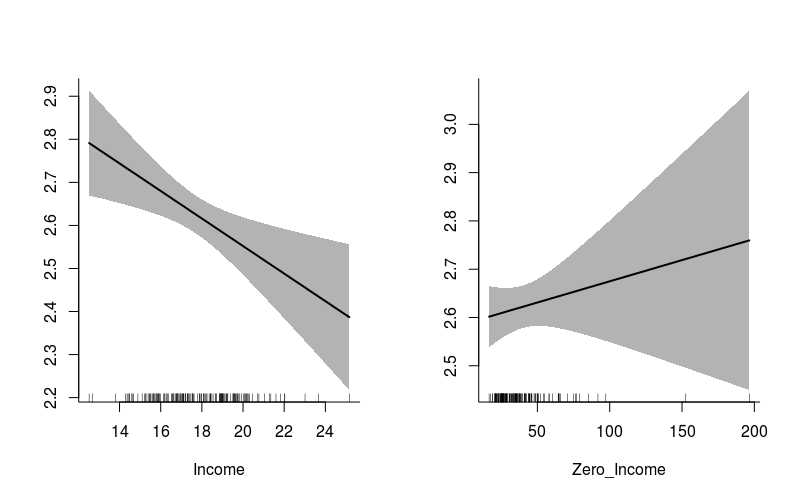
\includegraphics[width = 0.8\linewidth]{additive.png}
\caption{Section A.3: Plots of the fitted regression lines using semiparametric regression with Income and Zero Income as predictors. We can see that these predictors have a linear effect on the response variable crude birth rate (CBR) and hence splines are not necessary for these predictors and we can simply fit a parametric model to these predictors.}
\label{additive}
\end{figure}

\subsection{A.4}

As demonstrated in the previous section, a parametric model is sufficient for studying the relationship between Income, Zero Income and the response variable births per 1000. In this section we fit a Gamma GLM with the log link and wish to test whether the main effects model is sufficient and that adding interaction or higher order terms are not necessary at the 1\% level (which is taken to be the $\alpha$ for hypothesis testing). The reason for fitting the Gamma model in this case compared to Poisson for the previous case is due to lack of support for the Gamma family in the SemiPar R package. In the nonparametric case, we stick to the Poisson approximation whereas the GLM function allows us to fit a larger family from the exponential family of distributions. We fit two models in this section. The first model contains the main effects and has the following equation 
$$\text{log}(\text{birthsPer1000}_i) = \beta_0 + \beta_1\text{Income}_i + \beta_2\text{ZeroIncome}_i + \varepsilon_i $$ where $\varepsilon_i  \sim \text{Gamma}(k, \theta)$; (k: shape, $\theta$: scale) and the second model contains all second order terms. The equation for this is given below.

\begin{eqnarray*}
\text{log}(\text{birthsPer1000}_i) = \beta_0 + \beta_1\text{Income}_i + \beta_2\text{ZeroIncome}_i + \beta_3\text{Income}^2_i + \\
\beta_4\text{ZeroIncome}^2_i + \beta_5\text{Income}_i * \text{ZeroIncome}_i + \varepsilon_i
\end{eqnarray*}

where $\varepsilon_i  \sim \text{Gamma}(k, \theta)$; (k: shape, $\theta$: scale). For testing, we perform a likelihood ratio test between model 1 and model 2 since model 1 is nested in model 2. The null hypothesis $H_0$: model 1 is adequate vs the $H_a$: model 2 is adequate. The $p-$value for this is 0.32 (with $df=3$) which means that we cannot reject the null hypothesis at the 1\% level that model 2 is "better" than model 1, i.e., the data are more likely under model 2 than model 1. Thus, we can conclude that the data are almost equally likely under both models and hence, the additive model is sufficient for our purposes.\\

We also used the drop1 function in R which performs term-wise deletion and performs the likelihood ratio test between the models with the term included vs the model without the term (but all other terms in the model). This led to the same conclusion as the previous procedures in that dropping any of the second order terms does not change the log-likelihood by a significant amount and the models without the term are "as good as" the models with the term.

\subsection{A.5}

For this part we first fit a semiparametric model using spm in R package SemiPar. Income and Zero Income are included as parametric terms (of degree 1 as was shown in part A.3) and the rest of the terms are included in the non-parametric part. We dropped two predictors: population in January (which is highly correlated with population in December) and Nationality Out (countries to which people emigrated to) which is correlated with Nationality In. This was causing errors at the model fitting stage. Further, one could make the argument that we might be more concerned with nationals coming into Belgium than those going out of Belgium. We fit the model using the rest of the variables. Further, we include province as a random effect to account for the variability in different provinces.\\

Examining the fitted model, we see that the estimated degrees of freedom for all predictors except number of incoming international migrants is approximately 1 and for this variable is approximately 2.5. This means that a linear predictor for each of these predictors and a quadratic or cubic term for international incoming migrants may be sufficient and we can instead fit a parametric model instead of a semiparamteric one. We fit an initial model with all the predictors fit in the semiparametric model and include a quadratic as well as cubic term for number of incoming international migrants, and include province as a factor variable to potentially capture the mean shift in different provinces. Upon examining the coefficients, we narrow the set of predictors down to Income, Deaths, number of incoming and outgoing internal migrants, number of outgoing international migrants and the population in December. We fit a Gamma regression model in both cases with the log link function. A likelihood ratio test between these two models gives a $\chi^2= 18.359$ with $df_{full}-df_{reduced}=15$. The resulting $p-$value is 0.2443 so we decide to stick with the reduced model.\\ 

Another interesting comparison is whether the parametric model with knots that was fit in section A.2 can provide a better fit than this reduced model with quadratic and cubic effects for international incoming migrants. Since these models are non-nested, we can compare these two models based on their respective BIC values. the BIC for the reduced model is 726.84 and for the model with knots (at 400 and 1300) is 698.21. Based on this, we choose the model with the knots. The coefficients are given in table \ref{final-coeff}.\\

% latex table generated in R 3.2.5 by xtable 1.8-2 package
% Thu May 26 14:38:21 2016
\begin{table}[ht]
\centering
\begin{tabular}{ccccc}
  \hline
 Variables & Estimate & Std. Error & t value & Pr($>|$t$|$) \\ 
  \hline
(Intercept) & 2.6275 & 0.1216 & 21.60 & 0.0000 \\ 
  Income & -0.0174 & 0.0066 & -2.65 & 0.0089 \\ 
  Deaths & -0.0012 & 0.0003 & -3.78 & 0.0002 \\ 
  IntMig\_In & -0.0002 & 0.0001 & -1.48 & 0.1398 \\ 
  IntMig\_Out & 0.0002 & 0.0001 & 1.70 & 0.0918 \\ 
  IntlMig\_In & -0.0001 & 0.0001 & -0.77 & 0.4431 \\ 
  pmax((IntlMig\_In - 400), 0) & 0.0008 & 0.0002 & 4.87 & 0.0000 \\ 
  pmax((IntlMig\_In - 1300), 0) & -0.0007 & 0.0001 & -11.16 & 0.0000 \\ 
  IntlMig\_Out & -0.0004 & 0.0001 & -3.11 & 0.0023 \\ 
  Population\_Dec & 0.0000 & 0.0000 & 3.35 & 0.0010 \\ 
   \hline
\end{tabular}
\caption{Section A.5: Model summary for the final model in section A.5. This is a parametric model with piecewise linear terms for international incoming migrants by putting knots at (400, 1300) to capture the curvature in that variable.}
\label{final-coeff}
\end{table}

The interpretation for the coefficients is straightforward, however some of the coefficients appear to have a very small impact on the response variable. Income, as noted in one of the previous sections has a negative impact on the crude birth rate, i.e.\ families with higher income on average have lesser kids. Regions with a higher number of deaths appear to have a negative impact n the birth rates as well, possibly due to that region containing (on average) a higher number of elderly people. The slope for the incoming international migrants (between 0 and 400) is positive which could be due to regions with a smaller number of international migrants (more rural than urban) which would explain the slightly higher birth rate. For a region with a moderate amount of incoming international migrants (400-1300), the birthrates seem to decrease with an increase in the number of migrants. The number of outgoing international migrants seems to have a small negative impact on the birth rate as well. 

\section{Part B}

\subsection*{B.1: TIC for Poisson Regression}

In this section, we derive the formula for Takeuchi's information criterion for Poisson regression using the canonical link function: Y$_i \sim $ Poisson($\mu_i$) and $\mu_i = \text{exp}(x_i^t\beta) \Leftrightarrow \text{log}(\mu_i) = x_i^t\beta$. The log-likelihood of $\beta$ is given as:
\begin{align}
l(\beta) = \text{log}\mathcal{L}(\beta) = \sum_{i = 1}^n y_i \text{log}(\mu_i) - \mu_i - \text{log}(y_i) = \sum_{i = 1}^n y_i(x_i^t\beta) - e^{(x_i^t\beta)} - \text{log}(y_i)
\end{align}

Taking the derivative w.r.t.\ $\beta$, we have
\begin{align}
\frac{\partial l(\beta)}{\partial(\beta)} = \sum_{i = 1}^n y_ix_i - e^{(x_i^t\beta)} x_i = \sum_{i = 1}^n \left(y_i - e^{(x_i^t\beta)}\right)x_i
\end{align}

which is the score equation (when equated with 0). Taking the second derivative of the log-likelihood w.r.t.\ $\beta$ we get
\begin{align}
\frac{\partial^2 l(\beta)}{\partial \beta \partial \beta^t} = \sum_{i = 1}^n -e^{(x_i^t\beta)} x_i x_i^t
\end{align}

The equation for TIC is similar to AIC/BIC: $\text{TIC}(M) = -2 \text{log-likelihood}_{\text{max}}(M) + 2\text{Tr}(\hat{J}_n^{-1} \hat{K}_n)$ where $\hat{J}_n$ and $\hat{K}_n$ are given below by using the final terms from the derived equations (2.2) and (2.3) above
\begin{align}
\hat{J}_n = - \mathbb{E} \left[- \text{exp}(x_i^t \beta) x_i x_i^t \right] \quad \text{and} \quad \hat{K}_n = 
\mathbb{E} \left[ 
\left( (y_i - e^{(x_i^t\beta)}) x_i \right) 
\left( (y_i - e^{(x_i^t\beta)}) x_i \right)^t 
\right]
\end{align}

\subsection*{B.2: Simulation Study}
This part involves conducting a simulation study that compares AIC, BIC and TIC for Poisson regression. Five variables, $x_{i,j}$, $j = 2,\ldots,6$, $i = 1,\ldots,n$ were sampled from Uniform(-1,1). The response variable $Y$ was sampled from Poisson($\mu_i$) with $$\mu_i = \text{exp}\left(\frac{1}{3} + \frac{2}{3}x_{i,2} + 1*x_{i,3} + \frac{4}{3}x_{i,4} + 0*x_{i,5} + 0*x_{i,6}\right)$$
The response vector is $n$ x $1$ and the design matrix is an $n$ x $6$ matrix with the first column containing the intercept (all 1's) and the rest of the columns containing the $x_j$'s. Furthermore, we construct models with all the possible combinations of the covariates (which for 5 covariates results in $2^5=32$ models) and add the intercept term to each of the models. This simulation is run 1000 times for two sample sizes: $n=50$ and $n=400$ (table \ref{B2}). The aim is to see which models are selected and with what frequency by AIC, BIC and TIC (i.e.\, picking a model with the smallest (A/B/T)IC value). The results are presented below. 

% n = 50
\begin{table}[h]
	\begin{minipage}{.5\linewidth}
		\centering
			\begin{tabular}{c|c|c|c}
\hline
 Model & AIC & BIC & TIC \\
\hline
Only $\beta_1, \beta_2, \beta_3, \beta_4$ & 697 & 872 & 523\\
\hline
\thead{At least one of \\ $\beta_1, \beta_2, \beta_3, \beta_4 = 0$} & 15 & 49 & 11 \\
\hline
\thead{At least one of \\ $\beta_5, \beta_6 \neq 0$} & 288 & 79 & 466 \\
\hline
			\end{tabular}
		\caption*{(a) $n=50$}
	\end{minipage}
	\begin{minipage}{.5\linewidth}
		\centering
			\begin{tabular}{c|c|c|c}
\hline
 Model & AIC & BIC & TIC \\
\hline
Only $\beta_1, \beta_2, \beta_3, \beta_4$ & 723 & 971 & 692 \\
\hline
\thead{At least one of \\ $\beta_1, \beta_2, \beta_3, \beta_4 = 0$} & 0 & 0 & 0 \\
\hline
\thead{At least one of \\ $\beta_5, \beta_6 \neq 0$} & 277 & 29 & 308\\
\hline
			\end{tabular}
		\caption*{(b) $n=400$}
	\end{minipage}
\caption{Section B.2: Result for Poisson regression with $n=50$ and $n=400$ and 1000 simulations. The table entries show the number of times (out of 1000) that a particular model was selected having the smallest IC value.}
\label{B2}
\end{table}

Based on the simulations, it is observed that BIC tends to pick the correct model more than AIC or TIC for both small (50) and moderate (400) sample sizes. This demonstrates the strong consistency of BIC (it almost surely selects the correct underlying model) All three methods were correctly able to conclude the non-zero effect of $\beta_j$, j = 1,...,4 at moderately larger sample size. The tendency of AIC to overfit is well known and is observed in table \ref{B2} at both sample sizes where it selects the model with $\beta_5 \neq 0$  or $\beta_6 \neq 0$ which is known to be redundant due to the simulation setup. Larger sample size leads to a small decrease in this number, however.

\section{Part C}

This part involves using a high dimensional data set (71 x 4089) to identify the subset of genes (out of 4088, 1 column is the response) that play a role in the production of vitamin B2. Since $p>>n$, a majority of the regression approaches will not be possible and approaches that can deal with the high dimensional nature of the problem will be necessary. For this part, we first split up the data into training ($n=61$) and test sets ($n=10$). The models are fit to the training set and the average of the squared prediction error (MSPE) on the test set is computed (i.e. the square of the difference(s) between the values predicted by the model and the observed values). A "good" model in this case should induce sparsity (the most important predictors are identified; important can be defined as coefficients having the largest point estimates) and having the lowest MSPE on the test set. Regression with the following penalties were tried: ridge ($\alpha = 0$), lasso ($\alpha = 1$), elastic net ($\alpha = 0.1, 0.2, \ldots, 0.9$) and adaptive lasso. Another thing to keep in mind is that multicollinearity is to be expected in our dataset with a very large number of variables and due to the nature of the problem.\\

For the adaptive lasso, we cannot use $\hat{\beta}_{\text{ols}}$ as starting values for the initial weights since these parameters cannot be estimated. However, Zou (2006, p.6) \cite{zou} mentions that any other estimator for $\hat{\beta}$ can be chosen. Thus, as initial weights we choose $\hat{\beta}_{\text{ridge}}$ and the corresponding weights then become $w_i = 1/|\beta_i|^\gamma$ where $\gamma = 0.5$ is chosen arbitrarily (restriction: $\gamma>0$). This weight function ensures that coefficients with larger weights are penalized more and coefficients with smaller weights are penalized less. This is different from the lasso which penalizes all the coefficients equally.\\

The drawbacks of ridge and lasso are well known, namely that ridge regression does not induce sparsity as it continuously shrinks the coefficients towards zero without setting any of them to zero. Furthermore, if the variables are highly correlated, then lasso selects one out of the group of correlated variables and sets the rest to zero. In such a situation, elastic net usually gives more stable results.\\

For the models we fit, we are interested in two main parameters (apart from the usual regression parameters), namely the elastic net parameter $\alpha \in [0,1]$ and the regularization parameter $\lambda$ that keeps the size of the coefficients bounded. As mentioned above, $\alpha$ is evaluated for different values and for each $alpha$, we first pick a value for $lambda$ using $k$-fold cross-validation ($k=5$ in our case) on the training set that results in the smallest MSPE from a sequence of $lambda$ values. Next, we extract the coefficients for the model at this $lambda$ value and use these coefficients to calculate the MSPE on the test set. It should be noted that the $k$-fold CV is random as the folds are created randomly, however, if the model is truly able to capture the underlying relationship there should not be large variability across multiple runs. Table \ref{highdim} presents the results from this process.\\

\begin{table}[ht]
\centering
\begin{tabular}{c|ccccc}
  \hline
 & alpha & MSPE & lambda\_min & lambda\_1se & \thead{num\_coef \\ (incl/ intercept)} \\ 
  \hline
  1 (ridge) & 0.00 & 0.19 & 7.15 & 31.66 & 4089 \\
  \hline 
  2 & 0.10 & 0.12 & 0.29 & 1.06 & 144 \\ 
  3 & 0.20 & 0.11 & 0.20 & 0.33 &  94 \\ 
  4 & 0.30 & 0.11 & 0.10 & 0.22 &  77 \\ 
  5 & 0.40 & 0.11 & 0.07 & 0.14 &  69 \\ 
  6 & 0.50 & 0.12 & 0.08 & 0.18 &  55 \\ 
  7 & 0.60 & 0.14 & 0.01 & 0.24 &  78 \\ 
  8 & 0.70 & 0.12 & 0.03 & 0.20 &  54 \\ 
  9 & 0.80 & 0.12 & 0.07 & 0.23 &  40 \\ 
  10 & 0.90 & 0.14 & 0.01 & 0.13 &  58 \\
  \hline 
  11 (lasso) & 1.00 & 0.12 & 0.03 & 0.06 &  39 \\ 
  \hline
  \thead{adaptive \\ lasso} & 1.00 & 0.11 & 0.13 & - & 26 \\
   \hline
\end{tabular}
\caption{Section C: MSPE on the test set for different values of the elastic net penalty $\alpha \in [0,1]$. lambda\_min is the value of the regularization parameter $\lambda$ chosen by $k$-fold cross-validation. The last column displays the number of non-zero coefficients in the model selected for the corresponding alpha and lambda values.}
\label{highdim}
\end{table}

Based on these results, we first observe that there is not that much difference in the MSPE for all the models except for the ridge regression fit. Since the prediction errors are very similar, we can perhaps pick parsimony as a criterion for selection and pick the model with the adaptive lasso penalty as our final model. There is quite a large difference between the number of coefficients in the adaptive lasso solution and the elastic net solutions. Whether this model is truly better (which would imply that we are choosing to ignore the small but non-zero effects of the other genes picked by the larger models) would require further assessment. However, on the basis of MSPE and Occam's razor, we pick the model using adaptive lasso as the final model. The coefficients from the adaptive lasso fit are provided in the Appendix \ref{coeff}. The interpretation of the coefficients might be straightforward as in the usual regression case, however, the variable names are not particularly informative for somebody lacking domain-knowledge.

\begin{thebibliography}{1}

\bibitem{zou} Zou, H. (2006). The adaptive lasso and its oracle properties. \emph{Journal of the American statistical association}, 101(476), 1418-1429.

%\bibitem{lasso} Tibshirani, R. (1996). Regression shrinkage and selection via the lasso. \emph{Journal of the Royal Statistical Society. Series B (Methodological)}, 267-288.

\end{thebibliography}

\begin{comment}
\section{Appendix} \label{coeff}

Coefficients from the final model estimated in Part C.

\begin{table}[ht]
\centering
\begin{tabular}{|c|c|}
\hline
Variables &  Coefficients \\
\hline
(Intercept) & -13.5339     \\
x.AADK\_at  &   0.6148    \\
x.CARA\_at  &  -0.1134    \\
x.DEGA\_at  &  0.1720    \\
x.FLHP\_at  & 0.1838    \\
x.LYSC\_at  &  -0.2296    \\
x.RIBT\_at  &   0.2358    \\
x.XHLA\_at  &   0.0074    \\
x.XKDC\_at  &   0.5901    \\
x.XSA\_at   &  -0.4354    \\
x.YCLC\_at  &   0.0861    \\
x.YDBI\_at  &   0.0517    \\
x.YDBM\_at  &  -0.1313    \\
x.YDDK\_at  &  -0.0200    \\
x.YDDM\_at  &  -0.0489    \\
x.YFHE\_r\_at &  0.4319   \\
x.YFIQ\_at  &   0.1879    \\
x.YHDS\_r\_at &  0.1243   \\
x.YHDT\_at  &   0.0601    \\
x.YISU\_at  &   0.1121    \\
x.YOAC\_at  &  -0.3000    \\
x.YRPE\_at  &  -0.1700    \\
x.YURR\_at  &   0.2297    \\
x.YWPC\_at  &  -0.0944    \\
x.YXLC\_at  &  -0.3236    \\
x.YYCR\_at  &  -0.3386   \\
\hline
\end{tabular}
\caption{Section C: Estimated coefficients for the final model selected using the adaptive lasso.}
\label{final_model}
\end{table}
\end{comment}

\section{R Code}

\textbf{Note: The $\%>\%$ operator (used in the following R snippets) from the package "magrittr" makes it easier to read code.}

\subsection{Part A}

\begin{lstlisting}[language = R, frame = single]
library(dplyr); library(magrittr); library(splines); library(SemiPar); library(mgcv)

fulldata.A = read.table("/home/ad/Desktop/KUL Course Material/Statistical Modelling/Assignment/Examdata2016-A.txt", header = T)
set.seed(475672)
rownumbers = sample(1:589,size = 150)
mydata.A = fulldata.A[rownumbers,]

mydata.A %<>% mutate(province = floor(mydata.A[,1]/10000) + 9*(floor(mydata.A[,1]/1000) == 21) + 8*(floor(mydata.A[,1]/1000) == 25)) 

fulldata.A %<>% mutate(province = floor(fulldata.A[,1]/10000) + 9*(floor(fulldata.A[,1]/1000) == 21) + 8*(floor(fulldata.A[,1]/1000) == 25))

mydata.A = mydata.A[sort.list(mydata.A$IntlMig_In),]

# Part A.1
province_name = c("Antwerp", "Flemish Brabant", "West Flanders", "East Flanders", "Hainaut", "Liege", "Limburg", "Luxembourg", "Namur", "Walloon Brabant", "Brussels")

mydata.A %>% group_by(province) %>%  summarise(birthsPer1000 = mean(y), AvgIntl_in = mean(IntlMig_In))

mydata.A %>% group_by(province) %>% count(province)

# filter province 2 and 11
temp_df = filter(mydata.A, province %in% c(2,11)) %>% 
  dplyr::select(y, IntlMig_In, province) %>% 
  mutate(province = as.factor(province)) %>% arrange(province)

# wilcoxon test for testing the means of crude birth rate
wilcox.test(formula = y ~ province, conf.int = TRUE, data = temp_df)
wilcox.test(formula = IntlMig_In ~ province, conf.int = TRUE, data = temp_df)

# comparing against the whole dataset
fulldata.A %>% group_by(province) %>% count(province)

# filter province 2 and 11
temp_df_full = filter(fulldata.A, province %in% c(2,11)) %>% 
  dplyr::select(y, IntlMig_In, province) %>% 
  mutate(province = as.factor(province)) %>% arrange(province)

# wilcoxon test for testing the means of crude birth rate
wilcox.test(formula = y ~ province, conf.int = TRUE, data = temp_df_full)
wilcox.test(formula = IntlMig_In ~ province, conf.int = TRUE, data = temp_df_full)

# Part A.2
fit1 = spm(y ~ f(IntlMig_In), family = "poisson")
summary(fit1); plot(fit1); points(IntlMig_In, log(y_temp))

# can put knots at 50, 400, 1300 and 9500
fit_part = glm(y ~ IntlMig_In + pmax((IntlMig_In - 50),0) + pmax((IntlMig_In - 400),0) + pmax((IntlMig_In - 1300),0) + pmax((IntlMig_In - 9500),0), family = Gamma(link = "log")); summary(fit_part); plot(fit_part)

drop1(fit_part, test = "LRT")
lrtest(update(fit_part, . ~ . - pmax((IntlMig_In - 50),0) - pmax((IntlMig_In - 9500),0)), fit_part)

# plotting the picewise linear model on the spline fit
plot(fit1, ylim = c(2,3.2), xlab = "Number of Incoming International Migrants", ylab = "log(Expected birth rate per 1000)", lwd = 2)
points(IntlMig_In, log(y))
lines(IntlMig_In, log(fit_part$fitted.values), col = "green", lwd = 3)
abline(v = c(50, 400, 1300, 9500), lty = 2, lwd = 2)
legend(2800, 2.4, legend = c("Penalized Spline (33 knots)", "Linear spline w/ 4 knots (no penalization)"), col = c("black", "green"), lwd = c(2,3), lty = c(1,1)); title(main = "knots at 50, 400, 1300, 9500")

BIC(fit_part)
BIC(update(fit_part, . ~ . - pmax((IntlMig_In - 50),0) - pmax((IntlMig_In - 9500),0)))

# Part A.3
fit_additive = spm(y ~ f(Income, basis = "trunc.poly") + f(Zero_Income, basis = "trunc.poly"), family = "poisson"); summary(fit_additive); par(mfrow = c(1,2)); plot(fit_additive)

# Part A.4
fit_glm_add = glm(y ~ Income + Zero_Income, family = Gamma("log"))
fit_glm_full = glm(y ~ Income + Zero_Income + Income:Zero_Income + I(Income^2) + I(Zero_Income^2), family = Gamma("log"))
summary(fit_glm_add); summary(fit_glm_full)

library(lmtest)

lrtest(fit_glm_add, fit_glm_full)
drop1(fit_glm_full, scope = ~Income:Zero_Income + I(Income^2) + I(Zero_Income^2), test = "LRT")

# Part A.5
# fitting splines using spm
fit_all = spm(y ~ Income + Zero_Income + f(Density) + f(Marriages) + f(Divorces) + f(Deaths) + f(IntMig_In) + f(IntMig_Out) + f(IntlMig_In) + f(IntlMig_Out) + f(Nationality_In) + f(Population_Dec), family = "poisson", random = ~1, group = province); summary(fit_all); plot(fit_all, jitter.rug = TRUE)

# fitting splines using gam
fit_all_gam = gam(y ~ s(Income) + s(Zero_Income) + s(Density) + s(Marriages) + s(Divorces) + s(Deaths) + s(IntMig_In) + s(IntMig_Out) + s(IntlMig_In) + s(IntlMig_Out) + s(Nationality_In) + s(Population_Dec) + s(province), family = Gamma("log")); summary(fit_all_gam); plot(fit_all_gam)

# fitting spm with one nonparamteric
fit_all_spm = spm(y ~ Income + Zero_Income + Density + Marriages + Divorces + Deaths + IntMig_In + IntMig_Out + f(IntlMig_In) + IntlMig_Out + Nationality_In + Population_Dec, family = "poisson", random = ~1, group = province)
summary(fit_all_spm)

# fitting parametric with quadratic and cubic
fit_final = glm(y ~ Income + Zero_Income + Density + Marriages + Divorces + Deaths + IntMig_In + IntMig_Out + IntlMig_In + I(IntlMig_In ^ 2) + I(IntlMig_In ^ 3) + IntlMig_Out + Nationality_In + Population_Dec + as.factor(province), family = Gamma("log")); summary(fit_final)

drop1(fit_final, test = "LRT")

# reduced model with a subset of predictors
fit_reduced = glm(y ~ Income + Deaths + IntMig_In + IntMig_Out + IntlMig_In + I(IntlMig_In ^ 2) + I(IntlMig_In ^ 3) + IntlMig_Out + Population_Dec, family = Gamma("log")); summary(fit_reduced)

lrtest(fit_reduced, fit_final)

# model with knots instead of quadratic and cubic effects
fit_reduced2 = glm(y ~ Income + Deaths + IntMig_In + IntMig_Out + IntlMig_In + pmax((IntlMig_In - 400),0) + pmax((IntlMig_In - 1300),0) + IntlMig_Out + Population_Dec, family = Gamma("log")); summary(fit_reduced2)

BIC(fit_reduced); BIC(fit_reduced2)
\end{lstlisting}

\subsection{Part B}

\begin{lstlisting}[language = R, frame = single]
set.seed(475672)
# num of samples
n = 400 # 50, 400
# number of simulations
nsim = 1000
# list to store the final results
final50 = list()
final400 = list()

# simulation code
for (i in 1:nsim) {

x2 = runif(n, -1, 1); x3 = runif(n, -1, 1); x4 = runif(n, -1, 1); x5 = runif(n, -1, 1); x6 = runif(n, -1, 1)
mu_i = (1/3) + ((2/3) * x2) + x3 + ((4/3) * x4) + (0 * x5) + (0 * x6)
y = rpois(n, exp(mu_i))
des_mat = data.frame(Int = 1, x2, x3, x4, x5, x6)
# creating the combinations of variables
L = 5
combinations = function(L){
  comb = NULL
  for (i in 1:L) {comb = rbind(cbind(1,comb),cbind(0,comb))}
  return(comb)
}

# models to be fit
combination = cbind(1, combinations(5))
aic = c()
bic = c()
tic = c()
form = c()

for (k in seq_along(1:2 ^ L)) {
  
  temp_df = des_mat[,combination[k,] > 0]
  
  # this block is included because when k = 2^L only the intercept term is in the model in which case temp_df returns a vector and not a data frame so we can fit this manually for the last iteration; stupid edge cases
  if (k == 2 ^ L) { formulae = "y ~ 1"
    fit1 = glm(formulae, family = poisson)
  } else{ 
  	formulae = temp_df %>% names() %>% paste(collapse = " + ") %>%
      paste("y ~ 0 + ", ., sep = "")
    fit1 = glm(formulae, data = temp_df, family = poisson)
  }
  
  aic[k] = AIC(fit1)
  bic[k] = BIC(fit1)
  form[k] = formulae
  
  # calculating TIC
  # use y = y and x = temp_df
  temp_df %<>% as.matrix()
  beta_est = fit1$coefficients %>% as.matrix()
  mu_i_est = (temp_df %*% beta_est) %>% exp()
  
  first_deriv = (temp_df * as.vector((y - mu_i_est))) %>% as.matrix()
   
  Kmatrix = (t(first_deriv) %*% first_deriv)/n # p x p matrix
  
  # I(\beta) = (X^T)(D(\beta))(X)
  # where D(\beta) = the diagonal matrix with mu_i_est on the diagonal elements
  # (Observed) Fisher Information Matrix - p x p matrix
  Jmatrix = (t(temp_df) %*% diag(as.vector(mu_i_est)) %*% temp_df)/n 
  
  penaltyTIC = (solve(Jmatrix) %*% Kmatrix) %>% diag() %>% sum()
  
  tic[k] = (-2 * c(logLik(fit1))) + (2 * penaltyTIC)  
}

results = data.frame(Model = form, AIC = aic, BIC = bic, TIC = tic)
bestAIC = results %>% filter(AIC == min(AIC)) %>% select(Model, AIC)
bestBIC = results %>% filter(BIC == min(BIC)) %>% select(Model, BIC)
bestTIC = results %>% filter(TIC == min(TIC)) %>% select(Model, TIC)

if (n == 50) { 
  final50$modelAIC[i] = as.character(bestAIC$Model)
  final50$AIC[i] = bestAIC$AIC
  final50$modelBIC[i] = as.character(bestBIC$Model)
  final50$BIC[i] = bestBIC$BIC
  final50$modelTIC[i] = as.character(bestTIC$Model)
  final50$TIC[i] = bestTIC$TIC
} 

if (n == 400) { 
  final400$modelAIC[i] = as.character(bestAIC$Model)
  final400$AIC[i] = bestAIC$AIC
  final400$modelBIC[i] = as.character(bestBIC$Model)
  final400$BIC[i] = bestBIC$BIC
  final400$modelTIC[i] = as.character(bestTIC$Model)
  final400$TIC[i] = bestTIC$TIC
}

stopifnot(n != 50 || n != 400)
}

## analyzing the results
# n = 50
table(final50$modelAIC)
table(final50$modelBIC)
table(final50$modelTIC)

# n = 400
table(final400$modelAIC)
table(final400$modelBIC)
table(final400$modelTIC)
\end{lstlisting}

\subsection{Part C}

\begin{lstlisting}[language = R, frame = single]
library(glmnet)
library(xtable)

fulldata.C = read.table("/home/ad/Desktop/KUL Course Material/Statistical Modelling/Assignment/Examdata2016-C.txt", header = T, sep = ",")
set.seed(475672)
rownumbers = sample(1:71,61,replace = F)
mytraining = fulldata.C[rownumbers,]
mytest = fulldata.C[-rownumbers,]

# ridge regression for the coefficients to be used in adaptive lasso
ridge_cv = cv.glmnet(x = data.matrix(mytraining[,-1]), y = data.matrix(mytraining[,1]), nfolds = 5, alpha = 0, type.measure = "mse")
plot(ridge_cv)
ridge_cv$lambda.min

# variables for elastic net
alpha = seq(0, 1, 0.1)
mspe = c()
lambda_min = c()
lambda_1se = c()
num_coef = c()

for (i in seq_along(alpha)) {
  
  # fitting the model to the training set
  mod_cv = cv.glmnet(x = data.matrix(mytraining[,-1]), y = data.matrix(mytraining[,1]), nfolds = 5, alpha = alpha[i], type.measure = "mse")
  
  plot(mod_cv, main = paste("alpha = ", alpha[i], sep = ""))
  
  lambda_min[i] = mod_cv$lambda.min
  lambda_1se[i] = mod_cv$lambda.1se
  
  # getting the predictions on the test set
  pred = predict(mod_cv, newx = data.matrix(mytest[,-1]), s = "lambda.min") %>% as.vector()
  
  # mean of squared prediction errors
  mspe[i] = (mytest[,1] - pred) ^ 2 %>% mean()
  
  # number of coefficients in the selected model
  select_coef = coef(mod_cv, s = "lambda.min") %>% as.matrix()
  num_coef[i] = select_coef[select_coef != 0,] %>% length()
  
}

beepr::beep(3)

results = data.frame(alpha, MSPE = mspe,  lambda_min, lambda_1se, num_coef)
results

# adaptive lasso using glmnet and penalty factor
ridge_coef = coef(ridge_cv, s = "lambda.min") %>% as.matrix()
adapt_wt = 1/(abs(ridge_coef)) ^ 0.5

ada_lass = cv.glmnet(x = data.matrix(mytraining[,-1]), y = data.matrix(mytraining[,1]), alpha = 1, penalty.factor = adapt_wt, nfolds = 5, type.measure = "mse")
plot(ada_lass)
print(ada_lass)

# 0.1344 is the smallest lambda value chosen through print() and explains 92% of the variability in the response
pred = predict(ada_lass, newx = data.matrix(mytest[,-1]), s = 0.1344) %>% as.vector()
(mytest[,1] - pred) ^ 2 %>% mean()

ada_coef = coef(ada_lass, s = 0.1344) %>% as.matrix()

# which covariates are selected in the final model
ada_coef[ada_coef != 0,] %>% round(digits = 4)
\end{lstlisting}

\section{Appendix} \label{coeff}

Coefficients from the final model estimated in Part C.

\begin{table}[ht]
\centering
\begin{tabular}{|c|c|}
\hline
Variables &  Coefficients \\
\hline
(Intercept) & -13.5339     \\
x.AADK\_at  &   0.6148    \\
x.CARA\_at  &  -0.1134    \\
x.DEGA\_at  &  0.1720    \\
x.FLHP\_at  & 0.1838    \\
x.LYSC\_at  &  -0.2296    \\
x.RIBT\_at  &   0.2358    \\
x.XHLA\_at  &   0.0074    \\
x.XKDC\_at  &   0.5901    \\
x.XSA\_at   &  -0.4354    \\
x.YCLC\_at  &   0.0861    \\
x.YDBI\_at  &   0.0517    \\
x.YDBM\_at  &  -0.1313    \\
x.YDDK\_at  &  -0.0200    \\
x.YDDM\_at  &  -0.0489    \\
x.YFHE\_r\_at &  0.4319   \\
x.YFIQ\_at  &   0.1879    \\
x.YHDS\_r\_at &  0.1243   \\
x.YHDT\_at  &   0.0601    \\
x.YISU\_at  &   0.1121    \\
x.YOAC\_at  &  -0.3000    \\
x.YRPE\_at  &  -0.1700    \\
x.YURR\_at  &   0.2297    \\
x.YWPC\_at  &  -0.0944    \\
x.YXLC\_at  &  -0.3236    \\
x.YYCR\_at  &  -0.3386   \\
\hline
\end{tabular}
\caption{Section C: Estimated coefficients for the final model selected using the adaptive lasso.}
\label{final_model}
\end{table}

\end{document}